\documentclass[harvard]{lincolncsthesis}

%TC:ignore
% Packages you intend to use
% ..

% For example, if you want to render 
% the document in a different font you can
% use something like: 

% \usepackage{gentium}

\usepackage{url}
% Put the correct details in here
\author{Alfie Atkinson}
\studentnumber{25715017}
\email{25715017@students.lincoln.ac.uk}
\thesisDegree{Master of Science in Computer Science}
\thesisSubmissionDate{January 2025}

% If your thesis title spans over three lines, prepend the command with \Large!
\title{\bfseries\Large Evaluating the Attention-Based View in Risk Management and Proposing the New ``Top-Down'' Continuous and Proactive Security Assessment Model (CAPSAM)}

% Supervisor details
\thesisSupervisor{Dr. Saeid Pourroostaei Ardakani}
\thesisSecondSupervisor{Dr. Abimbola Sangodoyin}

\thesisLogoPath{figures/logo.pdf}  
% Add in the .bib files you wish to add 
% into your document here. If you want to
% include others, just copy this line and
% change the path!

\addbibresource{bib/references.bib}

\setlength{\parindent}{0.635cm}
\setlength{\parskip}{0pt plus 1pt}

\begin{document}

\maketitle

\begin{abstract}
    This paper evaluates the Attention-Based View (ABV) theory in the context of cybersecurity risk management and introduces a new model called the Continuous and Proactive Security Assessment Model (CAPSAM). The ABV theory suggests that a firm's behaviour is shaped by how decision-makers allocate their attention, with a focus on negative events such as high-cost cybersecurity breaches. While the ABV effectively explains why Top Management Teams (TMT) prioritise cybersecurity after a breach, it is limited by its reactive nature and does not address proactive security planning.
    
    CAPSAM, a ``top-down'' model, is designed to overcome these limitations by emphasising a proactive and continuous approach to risk assessment. The CAPSAM framework is built on five pillars: Culture, Continuous, Auditing, Response, and Proactive (CCARP), which integrates security considerations from the earliest stages of system development and throughout its lifecycle. The model operates within the FAMRM cycle, which stands for New Feature, Information Security Risk Assessment, Proactive Mitigation Strategies, Incident Response Planning, and Continuous Threat Monitoring, ensuring that security is embedded in every stage of a system's development.
    
    The paper argues that a top-down approach, prioritising executive leadership and strategic integration, is essential for establishing a strong security posture. This approach addresses the limitations of bottom-up strategies by aligning security initiatives with organisational goals and fostering a ``security-first mindset''. CAPSAM is theoretically grounded in the ABV, Agile and DevSecOps principles, ISO 31000 risk management standards, organisational learning, and stakeholder/trust theories. Real-world cases of major data breaches reinforce the need for such a proactive approach.
    
    CAPSAM's strengths include its proactive nature, continuous improvement cycle, and focus on customer data protection. The model also poses challenges, including the need for continuous updates, resource allocation, and consistent application across large organisations. The TMT plays a huge role in CAPSAM's implementation by championing security as a strategic objective and ensuring proper resource allocation. Overall, CAPSAM offers a robust framework that addresses the shortcomings of reactive security models and provides a comprehensive approach to cybersecurity.
\end{abstract}    

\thesisTables
\thesisBodyStart
%TC:endignore

\chapter{Introduction}
\section{Background on Cybersecurity Risks}
Cybersecurity is a rapidly growing field focused on safeguarding digital devices, networks, and information from unauthorised access and preventing data theft or alteration \citep{mijwil2023exploring}. It employs a range of techniques, processes, and practices to protect sensitive information and deter cyber attacks. Tactics for protecting against cyber attacks include firewalls, encryption, secure passwords, and threat detection and response systems, and employees should be trained on these strategies.

Cybersecurity risk is determined by the combination of vulnerabilities, threats, and the potential impact of cyber-attacks. Vulnerabilities are the weaknesses present in the system, and threats are the possibilities of cyber-attacks that exploit these vulnerabilities \citep{prasad2020cyber}. The Internet and the Internet of Things (IoT) are significant sources of threats, while phishing attacks are becoming increasingly sophisticated, and passwords alone are no longer sufficient for ensuring security. Raising awareness about cybersecurity risks is imperative for effectively handling digital environments and safeguarding them against electronic threats \citep{mijwil2023exploring}.

\section{The Role of Information Security Risk Assessments (ISRAs)}
Information Security Risk Assessments (ISRAs) are a key tool for identifying and managing vulnerabilities. ISRAs help organisations to identify their security risks and provide a measured analysis of their critical information assets, which informs the development of plans to mitigate these risks \citep{shedden2010information}. These assessments are essential for protecting IT assets and form the basis for a secure information system. \citet{shedden2010information} also say ISRAs enable organisations to prioritise their security efforts, focusing on the most important assets and vulnerabilities as well as helping organisations determine the most cost-effective way to reduce risks.

\section{Top Management Team (TMT) Involvement}
The Top Management Team (TMT) involvement is vital for effective risk management as they are ultimately responsible for ensuring that due diligence is undertaken in identifying risk and implementing effective systems of controls \citep{fazlida2015information}. TMT engagement can ensure that cybersecurity is viewed as an integral part of the organisation rather than a technical issue handled solely by IT. This involvement ensures a holistic approach to security, with the TMT championing risk assessment exercises and ensuring that cybersecurity receives the necessary resources and attention \citep{shaikh2023information}. \citet{fazlida2015information} also state that TMT attention to security is important to ensure that risk is reduced and the organisation meets its legal obligations.

\section{Purpose of the Report}
This report evaluates the use of the Attention-Based View (ABV) Theory by \citet{shaikh2023information}, exploring its strengths and limitations. The report will then introduce a new Continuous and Proactive Security Assessment Model (CAPSAM) as a solution. This model addresses the need for a proactive approach to cybersecurity, in contrast to the reactive focus of the ABV. The aim of this report is to critically appraise the ABV, revealing its shortcomings in proactive security planning, and then present CAPSAM as a proactive alternative.

\chapter{Case Study Paper – Appraisal of Theoretical Model and Hypothesis}
\section{Summary of the Case Study}
In the case study, \citet{shaikh2023information} ask: ``How do cybersecurity breach costs and Top Management Team (TMT) attention to cybersecurity influence a firm's decision to carry out an Information Security Risk Assessment (ISRA)?''. The research found that higher breach costs result in greater TMT attention to cybersecurity. Additionally, they find that TMT attention to cybersecurity partially mediates the relationship between breach costs and the decision to conduct an ISRA. Further elaborating that while an ISRA might sometimes be initiated by the cybersecurity function independently, the TMT plays a significant role in the decision, especially after high-cost breaches.

\section{Explanation of the Attention-Based View (ABV) Theory}
The case study uses the attention-based view (ABV) to explain how TMT attention is directed toward cybersecurity issues. The ABV theory suggests that firm behaviour is shaped by how decision-makers allocate their attention. This theory is built on the idea that human rationality is limited, and decision-makers must focus on specific issues to make effective choices. The ABV is composed of three key principles: focus of attention, structural distribution of attention, and situated attention.

    \subsection{Focus of Attention}
    The principle of the focus of attention explains that due to limited attention capacity, individuals prioritise issues based on their perceived importance and relevance within a given context. Senior managers must be selective about which issues they focus on because they cannot effectively attend to everything. Negative events such as high-cost cybersecurity breaches become salient, thus requiring TMT attention. This focus then dictates the actions decision-makers take.

    \subsection{Structural Distribution of Attention}
    The principle of structural distribution of attention posits that an individual's position within an organisation's hierarchy influences what they pay attention to. TMTs have a fiduciary duty to stakeholders to oversee and assess firm performance and must protect the firm's reputation. As the ultimate decision-makers, they are responsible for oversight. The TMT's hierarchical position means they are expected to pay closer attention to security issues, especially in the face of higher breach costs.

    \subsection{Situated Attention}
    The principle of situated attention argues that an individual's attention is a result of the immediate situation. Urgent issues, such as high-cost cybersecurity breaches that cause material damage to the firm, draw the focus of the TMT. While minor breaches might be handled by IT personnel, breaches with substantial financial or reputational consequences require managerial attention and follow-up.

\section{Statement of Hypotheses}
The case study tested the following four hypotheses related to the impact of cybersecurity breach costs and TMT attention on the decision to carry out an ISRA:
\begin{enumerate}
    \item Higher cybersecurity breach costs have a positive effect on the decision to carry out an ISRA.
    \item Higher cybersecurity breach costs have a positive effect on TMT attention to cybersecurity.
    \item TMT attention to cybersecurity has a positive effect on the decision to carry out an ISRA.
    \item TMT attention to cybersecurity mediates the positive effect of cybersecurity breach costs on the decision to carry out an ISRA.
\end{enumerate}

\section{Critical Appraisal of the ABV}

    \subsection{Merits/Strengths}
    The Attention-Based View (ABV) provides a strong framework for understanding why Top Management Team (TMT) attention to cybersecurity is heightened following a costly breach. The ABV effectively explains this through its core principles: focus of attention, structural distribution of attention, and situated attention. The focus of attention principle highlights how negative events like significant breaches become salient, compelling the TMT to prioritise cybersecurity, while the structural distribution of attention principle emphasises that the TMT's hierarchical position and fiduciary duty make them responsible for addressing major security failures. Situated attention further reinforces this by illustrating how immediate, severe breaches demand urgent managerial action.

    The ABV also explains why some firms might not act on security until a crisis emerges. According to the model (see Figure \ref{fig:ABV}), TMTs have a limited attention capacity and will only focus on issues that are deemed the most important. This limited attention capacity means that cybersecurity may not receive sufficient attention until a significant breach forces the TMT to recognise it as a priority. This is further supported by the idea that organisations may only react to failures rather than carry out preventive security measures due to difficulty in justifying security investments. The ABV also theorises that breaches can act as a learning opportunity, as they provide inputs to enhance the quality of future security risk assessments.

    \begin{figure}[htbp]
        \centering
        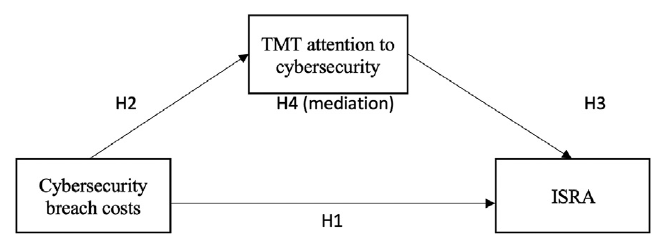
\includegraphics[width=0.8\textwidth]{figures/ABV-Theory.png}
        \caption{The Attention-Based View (ABV) Theory of TMT attention allocation, illustrating how breaches and organisational hierarchy influence decision-makers' focus \citep{shaikh2023information}.}
        \label{fig:ABV}
    \end{figure}

    \subsection{Demerits/Weaknesses}
    Despite its strengths, the ABV has some notable weaknesses. A significant limitation is that it primarily focuses on a reactive response to breaches, overlooking proactive security planning. The model is designed to explain how TMT attention is drawn to cybersecurity after a breach has occurred, but it does not adequately address how to prevent breaches in the first place. The ABV's emphasis on learning from failures shows its reactive stance, meaning that firms are continually playing catch up, rather than staying ahead of emerging threats.

    Additionally, the model assumes that TMT attention is driven primarily by negative events, ignoring other influences. While high-cost breaches undoubtedly capture the TMT's attention, \citet{gale2022governing} state that regulatory changes and industry standards are the most influential driver of board director's involvement in cybersecurity oversight. The ABV's narrow focus on breach-driven attention may lead to an incomplete understanding of the broader factors influencing security governance.

    Furthermore, the ABV does not provide a framework for proactive security measures. The model explains why TMTs react to breaches, but it offers little guidance on how to implement a security posture that anticipates threats. The model's focus on how the TMT reacts after a breach also overlooks the need for continuous monitoring, security by design, and other proactive strategies.

\section{Transition to New Model}
The limitations of the ABV indicate the need for a new, proactive model. While the ABV explains how firms respond to crises, a more comprehensive approach is required to prevent them. The next section will present a new model for information security risk assessment that shifts from a reactive to a proactive approach and addresses the limitations of the ABV. This new model is intended to help organisations implement security at every stage, rather than after they have already suffered a costly breach.

\chapter{New ``Top Down'' Model Selection for Information Security Risk Assessment}
\section{Introduction to the New Model}
This chapter introduces a new ``top-down'' Continuous and Proactive Security Assessment Model (CAPSAM) framework as a response to limitations in traditional risk assessment approaches. The case study by \citet{shaikh2023information} addressed the reactive nature of the Top Management Team (TMT)'s attention in its influence on the decision to carry out an Information Security Risk Assessment (ISRA). This reinforces the need for a new proactive, continuous security model that integrates information security across all layers of an organisation.

\section{Overview of the CAPSAM Framework}
    \subsection{Purpose, Goals, and Intended Outcomes}
    The CAPSAM framework is designed to \textbf{address the limitations of cybersecurity models} by emphasising a proactive and continuous approach to risk assessment. Its primary purpose is to \textbf{integrate information security considerations from the earliest stages of system development} and throughout its lifecycle.

    The main goal of CAPSAM is to minimise the likelihood and impact of cybersecurity breaches through vigilant, ongoing risk management. The model aims to \textbf{integrate information security across all layers of an organisation} and focuses on continuous improvement, ensuring a resilient security posture that adapts to the ever-changing threat landscape. By doing this, CAPSAM prioritises the protection of all stakeholders\textemdash including the customer and their data\textemdash strengthening overall organisational security and trust.

    \subsection{The Five Pillars of CAPSAM}
    The core philosophies of CAPSAM can be summarised in five pillars: \textbf{Culture, Continuous, Auditing, Response, Proactive (CCARP)}. These pillars are illustrated in Figure \ref{fig:CAPSAM} and form the foundation of the model's approach to information security risk management.

    \begin{figure}[htbp]
        \centering
        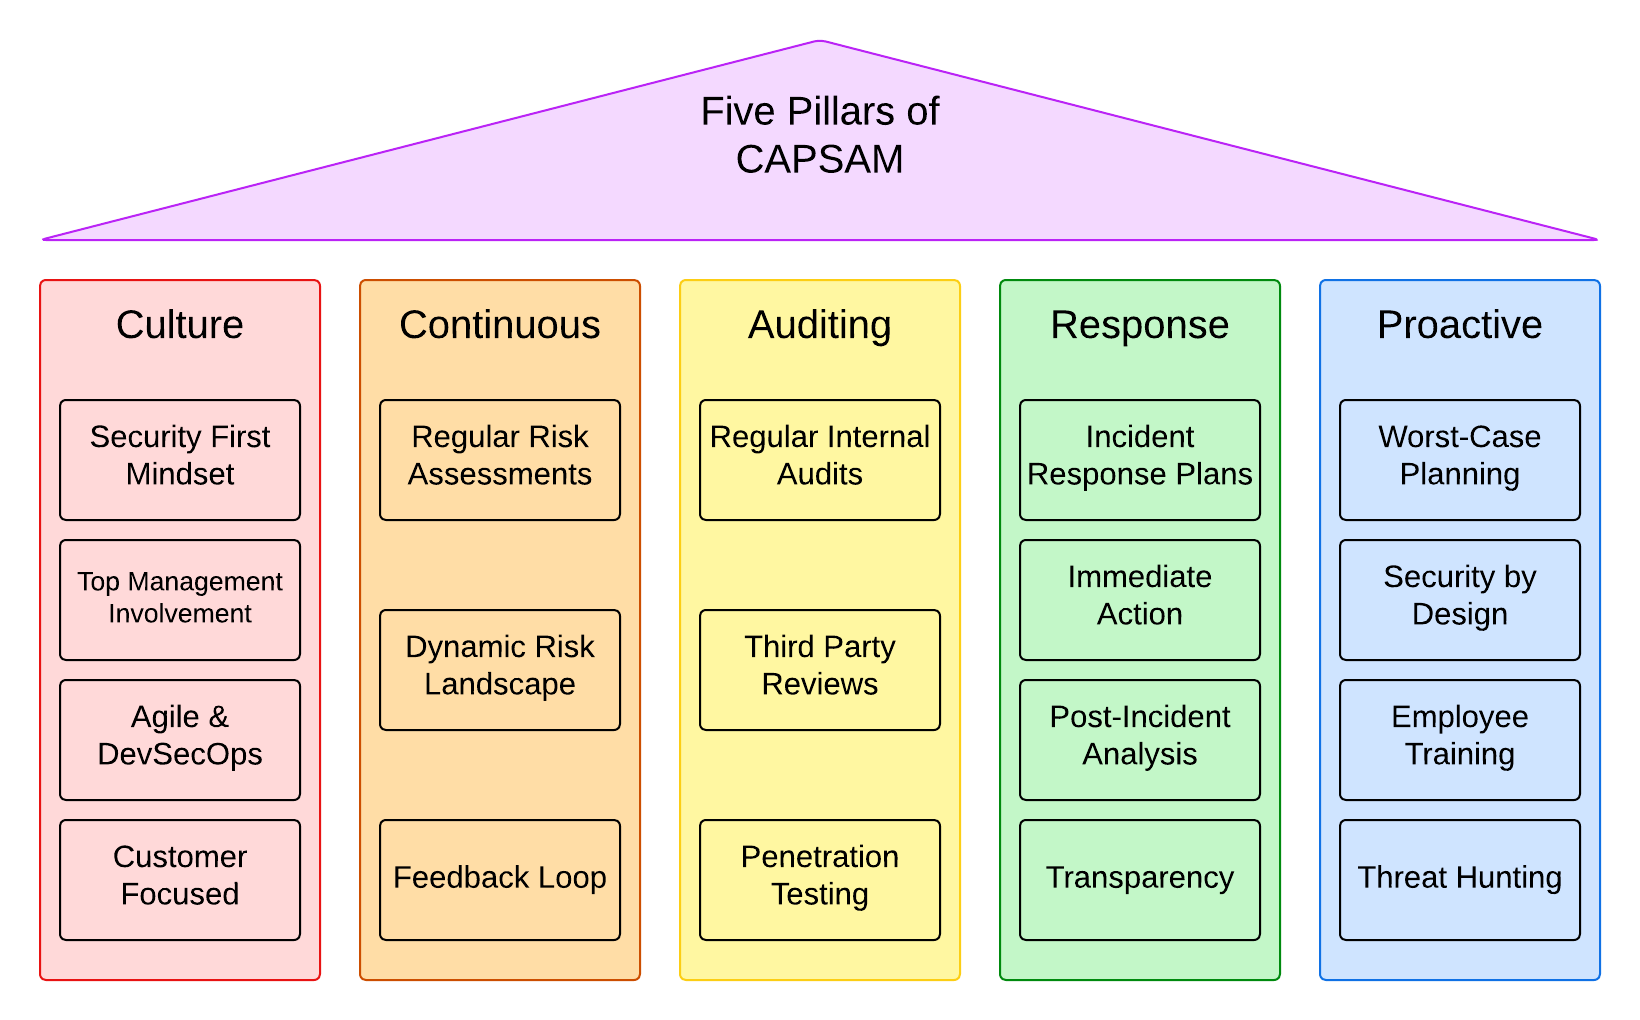
\includegraphics[width=0.8\textwidth]{figures/CAPSAM-Pillars.png}
        \caption{The Five Pillars of CAPSAM: Culture, Continuous, Auditing, Response, and Proactive (CCARP) and their components.}
        \label{fig:CAPSAM}
    \end{figure}

    \subsection{FAMRM Cycle}
    The CAPSAM framework operates within the FAMRM cycle (New \textbf{Feature}, Information Security Risk \textbf{Assessment}, Proactive \textbf{Mitigation} Strategies, Incident \textbf{Response} Planning, and Continuous Threat \textbf{Monitoring}). This cycle ensures that each new feature or system development is subject to proactive mitigation strategies, and continuous risk assessments where feedback loops inform the next ISRA. The FAMRM cycle is illustrated in Figure \ref{fig:FAMRM}.

    \begin{figure}[htbp]
        \centering
        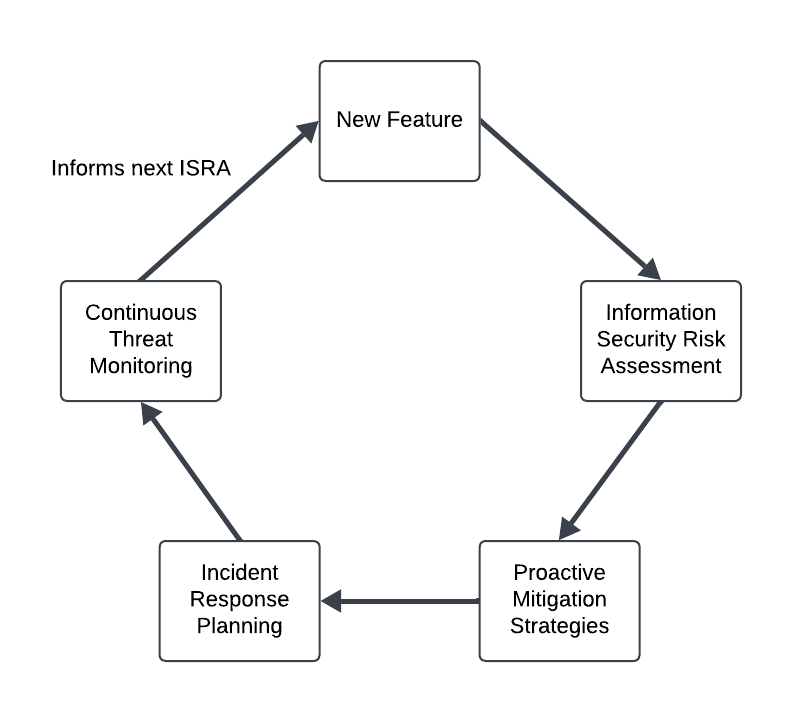
\includegraphics[width=0.6\textwidth]{figures/FAMRM-Cycle.png}
        \caption{FAMRM Cycle for Integrating Security into New Feature Development, Highlighting Continuous Risk Assessment, Proactive Mitigation, and Feedback Loops in Agile and DevSecOps Environments.}
        \label{fig:FAMRM}
    \end{figure}

\section{Justification for a Top-Down Approach}
    \subsection{Importance of Top-Down Risk Management}
    Explain the necessity of a top-down approach in information security risk management. Contrast this with the limitations of a bottom-up approach, which may be more reactive. Emphasize the need for executive engagement in setting priorities, allocating resources, and enforcing security policies.

    \subsection{Alignment with Corporate Governance}
    Discuss how a top-down approach aligns with corporate governance and strategic business objectives. Outline the benefits of ensuring top-level involvement in risk management processes.

    \subsection{Limitations of Bottom-Up Approaches}
    Describe the challenges of relying on bottom-up approaches, such as lack of management buy-in and difficulty in achieving holistic, coordinated efforts across departments.

\section{Theoretical Foundations}
    \subsection{Attention-Based View (ABV) and Proactive Security}
    Introduce the Attention-Based View theory, explaining its core concepts related to limited attention capacity for non-routine activities. Discuss how CAPSAM applies ABV to ensure information security is continuous and proactive.

    \subsection{Agile Methodology and DevSecOps Principles}
    Describe how agile methodologies and DevSecOps principles support continuous integration, delivery, and security practices. Relate this to CAPSAM’s focus on continuous feedback and improvement loops.

    \subsection{ISO 31000: Risk Management Standard}
    Discuss ISO 31000 and its relevance to CAPSAM. Emphasize how the risk management structure of ISO 31000 informs CAPSAM’s approach to risk analysis, evaluation, and treatment.

    \subsection{Organisational Learning and Continuous Feedback}
    Highlight the importance of continuous learning and feedback loops in CAPSAM. Connect this to principles of organisational learning and explain how feedback drives improvement in security measures.

    \subsection{Customer-Focused Approach and Trust Theory}
    Discuss how a customer-focused approach enhances trust and aligns with corporate social responsibility principles. Introduce trust theory and explain how it is integrated into CAPSAM to improve stakeholder engagement and organisational security.

\section{Critical Analysis and Justification}
    \subsection{Strengths of CAPSAM}
    Critically analyse the strengths of the CAPSAM model, such as its proactive nature, emphasis on stakeholder engagement, and its continuous improvement cycle. Use sources to support your claims on the benefits of proactive risk management.

    \subsection{Limitations of CAPSAM}
    Acknowledge the limitations and challenges of implementing CAPSAM. Discuss aspects such as the need for continuous updates to risk assessments, the resources required for ongoing monitoring, and the potential for over-reliance on specific teams or individuals.

    \subsection{Comparison with Case Study Approach}
    Compare CAPSAM with the reactive approach in the case study. Highlight how CAPSAM’s proactive, top-down, and continuous nature addresses the gaps and limitations of the case study approach.

    \subsection{Challenges in Implementing CAPSAM}
    Discuss potential challenges in implementing CAPSAM, such as obtaining management support, ensuring consistent communication across departments, and managing the resources needed for continuous monitoring.

\section{Implementation of CAPSAM}
    \subsection{Phase 1: Planning and Preparation}
    Outline the first phase of implementing CAPSAM, which involves identifying key stakeholders, defining roles and responsibilities, and establishing communication channels. Discuss the importance of aligning the security risk management policy with the organisation’s overall strategy.

    \subsection{Phase 2: Implementation}
    Describe the process of conducting risk assessments, identifying vulnerabilities, prioritizing risks, and developing mitigation strategies. Explain the importance of integrating risk management activities with the software development lifecycle.

    \subsection{Phase 3: Review and Improvement}
    Detail the review phase, which involves regular assessments of the CAPSAM framework, adapting the model based on insights and business changes, and fostering a culture of continuous security improvement.

\section{Conclusion}
Summarize the key points discussed in the chapter, reinforcing the value of the CAPSAM framework in overcoming the limitations of traditional risk assessment models. Emphasize the importance of a proactive, continuous approach to information security and its alignment with business practices and strategic goals.

\chapter{Conclusion}
\section{Summary of the Case Study Evaluation}
The case study effectively uses the ABV theory to explain how a significant cybersecurity breach captures the attention of the TMT. However, ABV is a reactive model, focusing on responses after a breach and lacking guidance on proactive measures. The model's emphasis on learning from failures highlights the need for a more comprehensive security governance approach, including prevention.

\section{Key Features of CAPSAM}
CAPSAM integrates security across an organisation through five core components: Culture (security-first mindset), continuous risk assessment, auditing (regular reviews), response plans for incidents, and a proactive approach (worst-case scenario planning). CAPSAM's iterative approach ensures a resilient security posture, offering a clear improvement over reactive models.

\section{Role of the TMT}
The TMT plays a crucial role in CAPSAM's success by championing security as a strategic objective and ensuring proper resource allocation. Unlike models that treat security as a technical issue, CAPSAM requires TMT involvement to create a security-first culture, making their commitment vital for effective implementation.

\section{Benefits of CAPSAM}
CAPSAM enhances cybersecurity by reducing the likelihood of successful cyberattacks through its proactive approach. Its continuous nature enables dynamic responses to emerging threats, ensuring resilience over time. By embedding security into all development stages, CAPSAM offers robust protection for organisational assets and consumer trust, making security a core component of the system and culture.

\printReferences

\printAppendices

\end{document}